%!TEX program = xelatex
\documentclass[dvipsnames,svgnames,a4paper,10pt]{article}

% -----------------------------------------------------
%	加边框的命令
%	参考：https://tex.stackexchange.com/questions/531559/how-to-add-the-page-border-for-first-two-pages-in-latex
\usepackage{tikz}
\usetikzlibrary{calc}
\usepackage{eso-pic}
\AddToShipoutPictureBG{%
\begin{tikzpicture}[overlay,remember picture]
\draw[line width=0.6pt] % 边框粗细
    ($ (current page.north west) + (0.6cm,-0.6cm) $)
    rectangle
    ($ (current page.south east) + (-0.6cm,0.6cm) $); % 边框位置
\end{tikzpicture}}


\usepackage{xcolor}
\definecolor{c1}{HTML}{2752C9} % 目录颜色
\definecolor{c2}{RGB}{190,20,83} % 引用颜色

\usepackage{ctex}
\usepackage[top=28mm,bottom=28mm,left=15mm,right=15mm]{geometry} % 调整边距
\usepackage{hyperref}
\hypersetup{
	colorlinks,
	linktoc = section, % 给目录加的超链接位置，选项有 section, page, all
	linkcolor = c1, % linkcolor 目录颜色
	citecolor = c1  % citecolor 引用颜色
}
\usepackage{amsmath,enumerate,multirow,float}
\usepackage{tabularx}
\usepackage{tabu}
\usepackage{subfig}
\usepackage{fancyhdr}
\usepackage{graphicx}
\usepackage{wrapfig}
\usepackage{physics}
\usepackage{appendix}
\usepackage{amsfonts,amssymb}
% \usepackage{annotate-equations} % 公式标注（未安装，已禁用）
\usepackage{pgfplots} % pgf 绘图


% ---------------------------------------------------------------------
%	定义了两类colorbox
\usepackage{tcolorbox}
\tcbuselibrary{skins,breakable}
\newtcolorbox{tbox}[2][]{
    colframe=black!70!,
    breakable,
    enhanced, % 跨页后不会显示下边框
    boxrule =0.5pt,
    title = {#2},
    fonttitle = \large\bfseries,
    drop fuzzy shadow,
    #1
}
\newtcolorbox[auto counter,number within=section]{question}[1][]{
  top=2pt,bottom=2pt,arc=1mm,
  boxrule=0.5pt,
  breakable,
  enhanced, % 跨页后不会显示下边框
  coltitle=c1!80!gray,
  colframe=c1,
  colback=c1!3!white,
  drop fuzzy shadow,
  title={思考题~\thetcbcounter：\quad},
  fonttitle=\bfseries,
  attach title to upper,
  #1
}

% ---------------------------------------------------------------------
%	利用 cleveref 改变引用格式，\cref 是引用命令
\usepackage{cleveref}
\crefformat{figure}{#2{\textcolor{c2}{图 #1}}#3} % 图片的引用格式
\crefformat{equation}{#2{(\textcolor{c2}{#1})}#3} % 公式的引用格式
\crefformat{table}{#2{\textcolor{c2}{表 #1}}#3} % 表格的引用格式

% ---------------------------------------------------------------------
%	页眉页脚设置
\fancypagestyle{plain}{\pagestyle{fancy}}
\pagestyle{fancy}
\lhead{\kaishu 中山大学物理与天文学院物理实验\uppercase\expandafter{\romannumeral3}} % 左边页眉，学院 + 课程
\rhead{\kaishu Template 实验报告模板} % 右边页眉，实验报告标题
\cfoot{\thepage} % 页脚，中间添加页码
\setlength{\headheight}{13.6pt}

% ---------------------------------------------------------------------
%	对目录、章节标题的设置
\renewcommand{\contentsname}{\centerline{\huge 目录}}
% titlesec/titletoc 与 ctex 冲突，已禁用
% \usepackage{titlesec}
% \usepackage{titletoc}
% \titleformat{\section}{\centering\LARGE}{}{1em}{}
% \newcommand{\nsection}[3]{%
%     \section{#1 #2 \hspace{11pt} \textbf{#3}}%
% }

% ---------------------------------------------------------------------
%   listing代码环境设置
\usepackage{listings}
\lstloadlanguages{python}
\lstdefinestyle{pythonstyle}{
backgroundcolor=\color{gray!5},
language=python,
frameround=tftt,
frame=shadowbox,
keepspaces=true,
breaklines,
columns=spaceflexible,
basicstyle=\ttfamily\small, % 基本文本设置，字体为 teletype，大小为 small
keywordstyle=[1]\color{c1}\bfseries,
keywordstyle=[2]\color{Red!70!black},
stringstyle=\color{Purple},
showstringspaces=false,
commentstyle=\ttfamily\scriptsize\color{green!40!black}, % 注释文本设置，字体为 teletype，大小为 scriptsize
tabsize=2,
morekeywords={as},
morekeywords=[2]{np, plt, sp},
numbers=left, % 代码行数，位置在左
numberstyle=\it\tiny\color{gray}, % 代码行数的数字字体设置
stepnumber=1,
rulesepcolor=\color{gray!30!white}
}


% ---------------------------------------------------------------------
%	将表格封装起来
\newcommand{\scoresTable}[8]{
    \begin{table}
        \renewcommand\arraystretch{1.7}
        \begin{tabularx}{\textwidth}{
                |X|X|X|X
                |X|X|X|X|}
            \hline
            \multicolumn{2}{|c|}{预习报告} & \multicolumn{2}{|c|}{实验记录} & \multicolumn{2}{|c|}{分析讨论} & \multicolumn{2}{|c|}{总成绩} \\
            \hline
            \centering#1&\centering#2 &\centering#3 &\centering#4 &\centering#5 &\centering#6 &\centering#7 &{\centering#8} \\
            \hline
        \end{tabularx}
    \end{table}
}
\newcommand{\infoTable}[6]{
    \begin{table}
        \renewcommand\arraystretch{1.7}
        \begin{tabularx}{\textwidth}{|X|X|X|X|}
        \hline
        专业：& #1 &年级：& #2\\
        \hline
        姓名：& #3   & 学号：&#4\\
        \hline
        实验时间：&#5 & 教师签名：&#6 \\
        \hline
        \end{tabularx}
    \end{table}
}

% ---------------------------------------------------------------------
%	其他设置
\def\degree{${}^{\circ}$} % 角度
\graphicspath{{./}{./images/}} % 插入图片的相对路径
\allowdisplaybreaks[4]  %允许公式跨页

\usetikzlibrary{patterns,decorations.markings,arrows.meta,bending} % TikZ 包的拓展

\pgfplotsset{compat=1.18}
\graphicspath{{./}{images/}}
\usepackage{booktabs}
\usepackage{makecell}
\usepackage{array}
\usepackage{enumitem}
\usepackage{caption}
\captionsetup{font=small,labelfont=bf}
\setlength{\parskip}{0.2em}
\setlength{\parindent}{2em}
\renewcommand{\arraystretch}{1.12}

\hypersetup{
  pdftitle={实验二：Fashion-MNIST 卷积分类与扩散生成},
  pdfauthor={赵浩宇}
}
\lhead{\kaishu 计算机视觉实验报告}
\rhead{\kaishu 实验二：Fashion-MNIST}

\begin{document}
\ClearShipoutPictureBG
\begin{titlepage}
\thispagestyle{empty}
\begin{center}
  \vspace*{0.25cm}
  
\includegraphics[width=0.40\textwidth]{images/school_flat.png}\par
  \vspace{0.55cm}
  {\fontsize{30pt}{36pt}\selectfont\bfseries 计算机视觉\par}
  \vspace{0.65cm}
  {\fontsize{28pt}{34pt}\selectfont\bfseries 实验报告\par}
  \vspace{1.6cm}
  {\fontsize{21pt}{30pt}\selectfont\bfseries 实验二：Fashion-MNIST\par}
  {\fontsize{18pt}{28pt}\selectfont\bfseries 卷积分类、结构先验与扩散生成\par}
\end{center}
\vspace{1.1cm}
\begin{center}
\renewcommand\arraystretch{1.75}
{\fontsize{17pt}{23pt}\selectfont
\begin{tabular}{p{0.22\textwidth}p{0.48\textwidth}}
学院： & \underline{\makebox[0.36\textwidth][c]{电子信息与通信学院}} \\
专业班级： & \underline{\makebox[0.36\textwidth][c]{电信2303班}} \\
姓名： & \underline{\makebox[0.36\textwidth][c]{赵浩宇}} \\
学号： & \underline{\makebox[0.36\textwidth][c]{U202314553}} \\
指导教师： & \underline{\makebox[0.48\textwidth][c]{王兴刚、廖振宇、闫增强}} \\
\end{tabular}}
\end{center}
\end{titlepage}

\begingroup
\renewcommand{\contentsname}{\centerline{\LARGE 目录}}
\small
\setcounter{tocdepth}{2}
\setlength{\parskip}{0pt}
\tableofcontents
\endgroup
\clearpage

\section{实验任务与模型设置}
Fashion-MNIST 含 28$\times$28 灰度服饰图像和 10 个类别\cite{fashionmnist}。本实验沿用实验 1 的官方训练集固定划分（50,000 训练、10,000 验证；split seed 42），官方测试集仅用于选定验证集检查点后的最终评价。分类模型均使用 $[0,1]$ 输入、不做随机增强；训练 30 epoch、batch size 128、Adam 学习率 $10^{-3}$、weight decay 0，训练种子为 42、123、2026。每个实验条件报告三种子测试准确率均值与样本标准差。

\subsection{结构与参数量}
MLP 沿用实验 1 的 $784\to128\to10$ ReLU 基线。CNN 使用两组 $3\times3$ 卷积、ReLU 与 $2\times2$ 最大池化，随后展平并接全连接分类头。尺寸按单样本列出；卷积参数包含 bias，ReLU、池化和展平不含参数。
\begin{table}[H]
\centering\small
\caption{网络层输出尺寸与可训练参数量}
\begin{tabular}{llrr}
\toprule
模型 & 层 & 输出尺寸 & 参数量 \\
\midrule
MLP & Flatten & 784 & 0 \\
 & Linear $784\to128$ + ReLU & 128 & 100,480 \\
 & Linear $128\to10$ & 10 & 1,290 \\
 & \textbf{总计} & & \textbf{101,770} \\
\midrule
CNN & 输入 & $1\times28\times28$ & 0 \\
 & Conv $1\to32$, $3\times3$, pad 1 + ReLU & $32\times28\times28$ & 320 \\
 & MaxPool $2\times2$ & $32\times14\times14$ & 0 \\
 & Conv $32\to64$, $3\times3$, pad 1 + ReLU & $64\times14\times14$ & 18,496 \\
 & MaxPool $2\times2$ & $64\times7\times7$ & 0 \\
 & Flatten & 3,136 & 0 \\
 & Linear $3136\to128$ + ReLU & 128 & 401,536 \\
 & Linear $128\to10$ & 10 & 1,290 \\
 & \textbf{总计} & & \textbf{421,642} \\
\bottomrule
\end{tabular}
\end{table}
CNN 参数量约为 MLP 的 4.14 倍，其中全连接 $3136\to128$ 层占 CNN 总参数约 95.2\%。因此本实验比较的是两种完整模型方案，性能差异不能只归因于卷积运算本身。

\section{卷积分类与结构先验检验}
\subsection{原图上的受控比较}
分类对照在每种子上使用相同的数据划分、训练轮数、优化器、批量大小与检查点规则；每轮按验证准确率保存最佳模型，测试集不参与选模。CNN 参数更多，但在当前设置下耗时与 MLP 接近。\cref{tab:cls} 给出汇总；耗时是当前服务器上的单次运行墙钟记录，不能直接视为跨硬件的计算复杂度。
\begin{table}[H]
\centering\small
\caption{原图与像素置换图上的分类结果（3 个种子，均值 $\pm$ 样本标准差）}
\label{tab:cls}
\begin{tabular}{llrrr}
\toprule
输入 & 模型 & 参数量 & 测试准确率 & 运行时间（秒） \\
\midrule
原图 & MLP & 101,770 & $0.8840\pm0.0012$ & $130.4\pm1.0$ \\
原图 & CNN & 421,642 & $0.9189\pm0.0034$ & $132.3\pm0.5$ \\
置换图 & MLP & 101,770 & $0.8859\pm0.0010$ & $151.9\pm1.5$ \\
置换图 & CNN & 421,642 & $0.8788\pm0.0023$ & $152.4\pm0.2$ \\
\bottomrule
\end{tabular}
\end{table}

原图上 CNN 比 MLP 高 3.48 个百分点；逐种子差值为 3.11、3.35、3.99 个百分点，方向一致。CNN 的召回率优势并非来自每一类都等幅提升：seed 42 上 Coat 与 Shirt 召回率分别为 0.822、0.740，仍较易与其他上装混淆；混淆矩阵中 Shirt 被判为 T-shirt/top 110 张，Coat 被判为 Pullover 80 张、被判为 Shirt 61 张。\cref{fig:cls} 展示训练过程，\cref{fig:err} 给出按测试索引先后出现的错误样本，未人工挑选成功案例。

为便于复核汇总统计，表中列出每个条件对应的三个独立训练种子结果。均值与样本标准差由这些原始准确率按条件分别计算；不同种子改变模型初始化和训练随机性，数据划分与像素置换保持固定。CNN 三个种子均优于 MLP，但三次差值（3.11--3.99 个百分点）并不相同。样本标准差描述有限的训练随机性，不是总体置信区间，三个种子不足以支持很强的显著性推断。训练曲线仅绘制 seed 42，是训练动态的代表性实例，表格则汇总三个种子。
\begin{table}[H]
\centering\small
\caption{各分类条件的逐种子测试准确率}
\label{tab:seed-accuracy}
\begin{tabular}{llrrr}
\toprule
输入 & 模型 & seed 42 & seed 123 & seed 2026 \\
\midrule
原图 & MLP & 0.8853 & 0.8839 & 0.8829 \\
原图 & CNN & 0.9164 & 0.9174 & 0.9228 \\
置换图 & MLP & 0.8860 & 0.8849 & 0.8868 \\
置换图 & CNN & 0.8766 & 0.8786 & 0.8811 \\
\bottomrule
\end{tabular}
\end{table}

\begin{figure}[H]
\centering
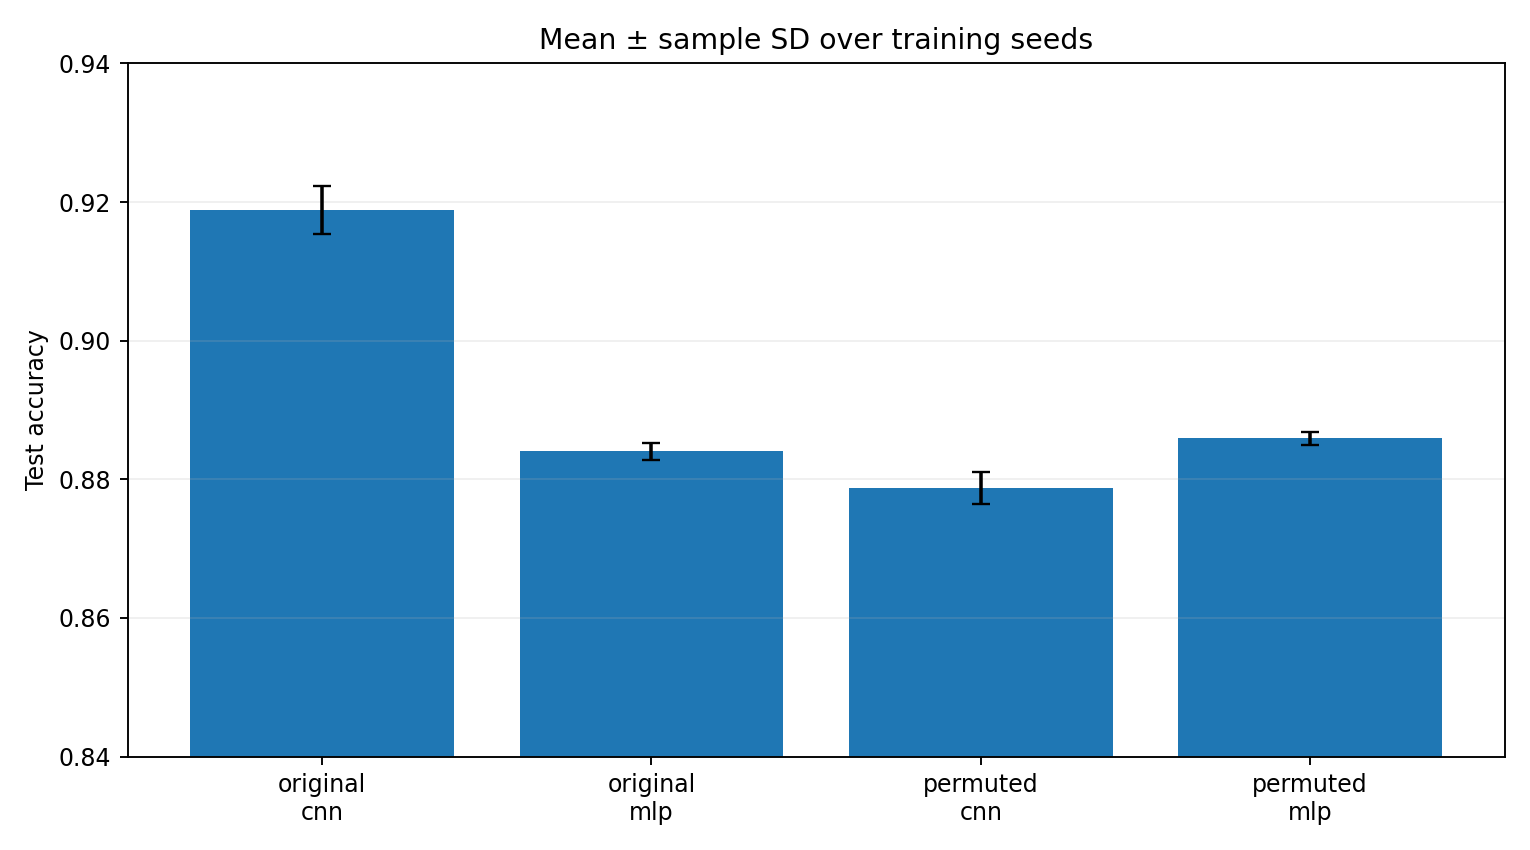
\includegraphics[width=0.48\textwidth]{images/exp2/comparison_mean_std.png}\hfill
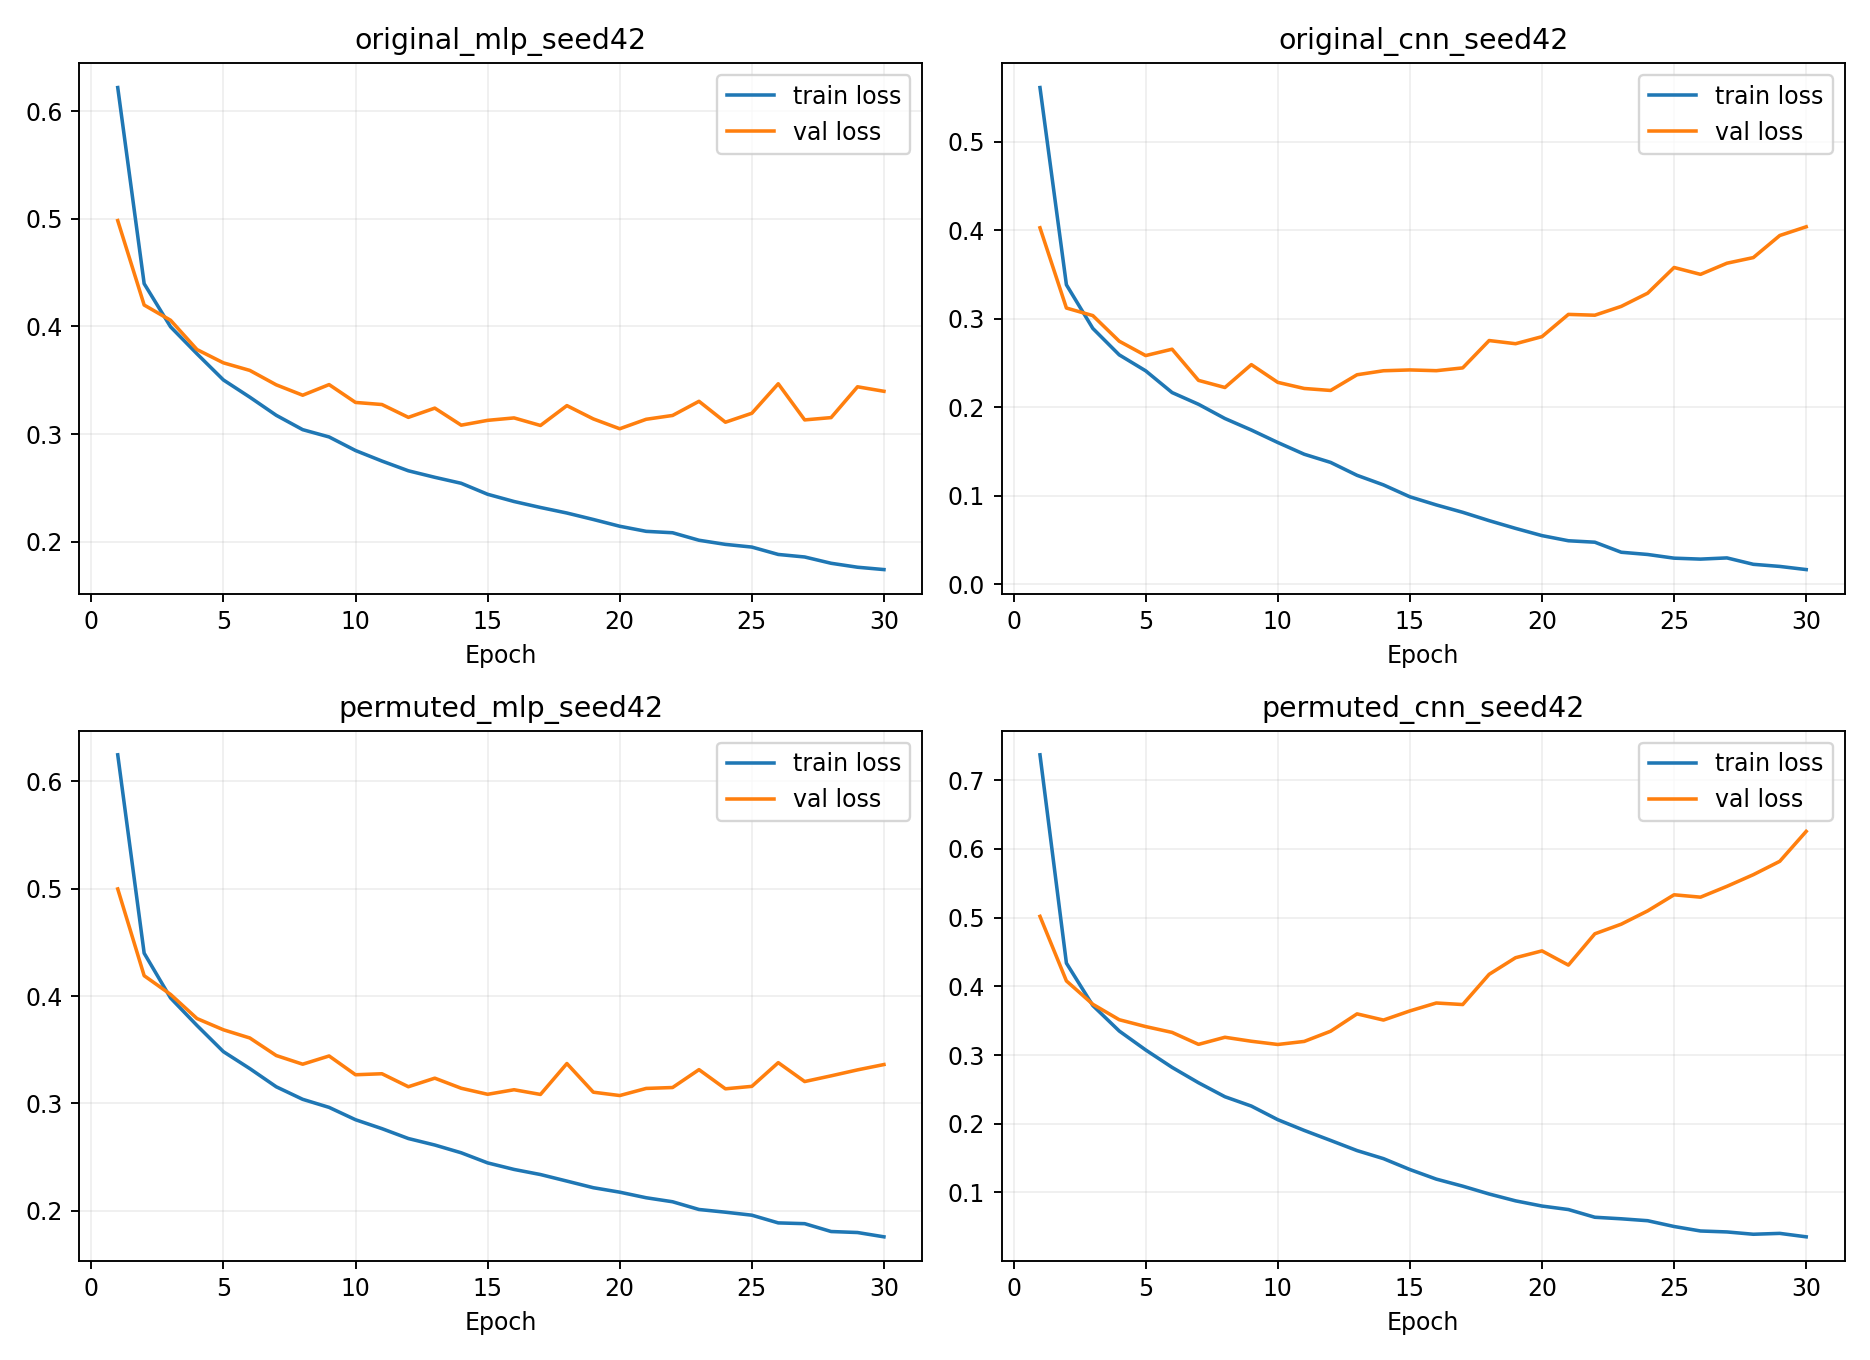
\includegraphics[width=0.48\textwidth]{images/exp2/classification_curves.png}
\caption{左：四种条件的测试准确率均值与样本标准差；右：seed 42 的训练/验证损失曲线（四个模型条件）}
\label{fig:cls}
\end{figure}
\begin{figure}[H]
\centering
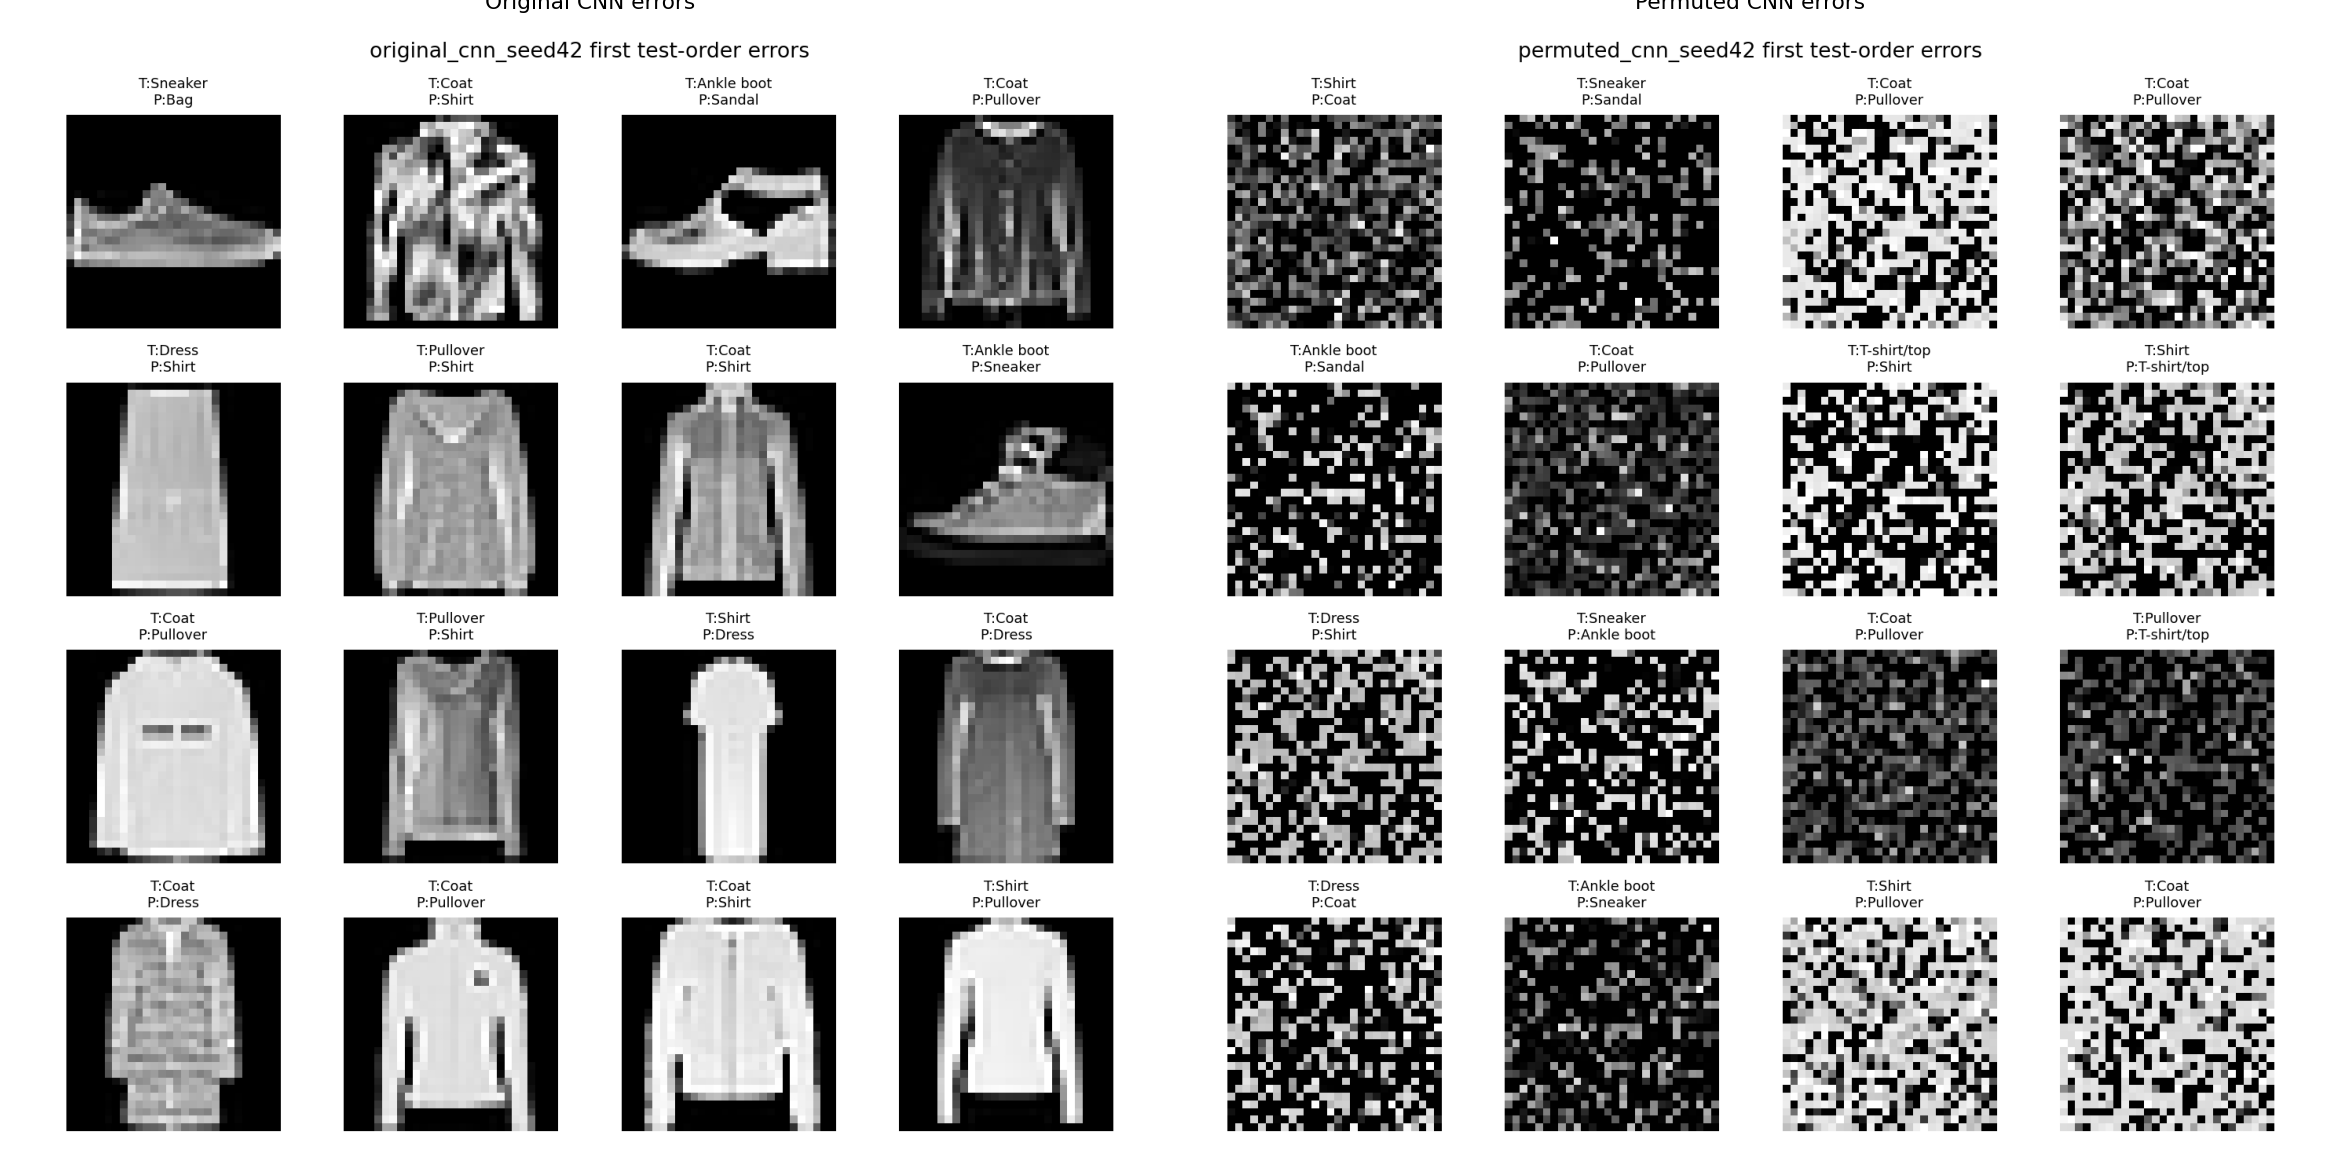
\includegraphics[width=0.92\textwidth]{images/exp2/cnn_errors_pair.png}
\caption{seed 42 的 CNN 测试错误：上为原图、下为像素置换图，各展示按测试索引顺序出现的前 16 个错误}
\label{fig:err}
\end{figure}

为了不只呈现 CNN 的错误，\cref{fig:mlp-errors} 给出相同种子下 MLP 的原图与置换图错误样本。错误图按照测试集索引由小到大展示前 16 个误分类，不按类别或置信度筛选。原图模式下模型仍能利用轮廓区分多数鞋类和包类，但上装类别边界模糊；置换后像素图失去可读的空间轮廓，因此图像本身不再支持直观语义归因，需结合混淆矩阵和召回率判断。
\begin{figure}[H]
\centering
\begin{minipage}{0.48\textwidth}\centering
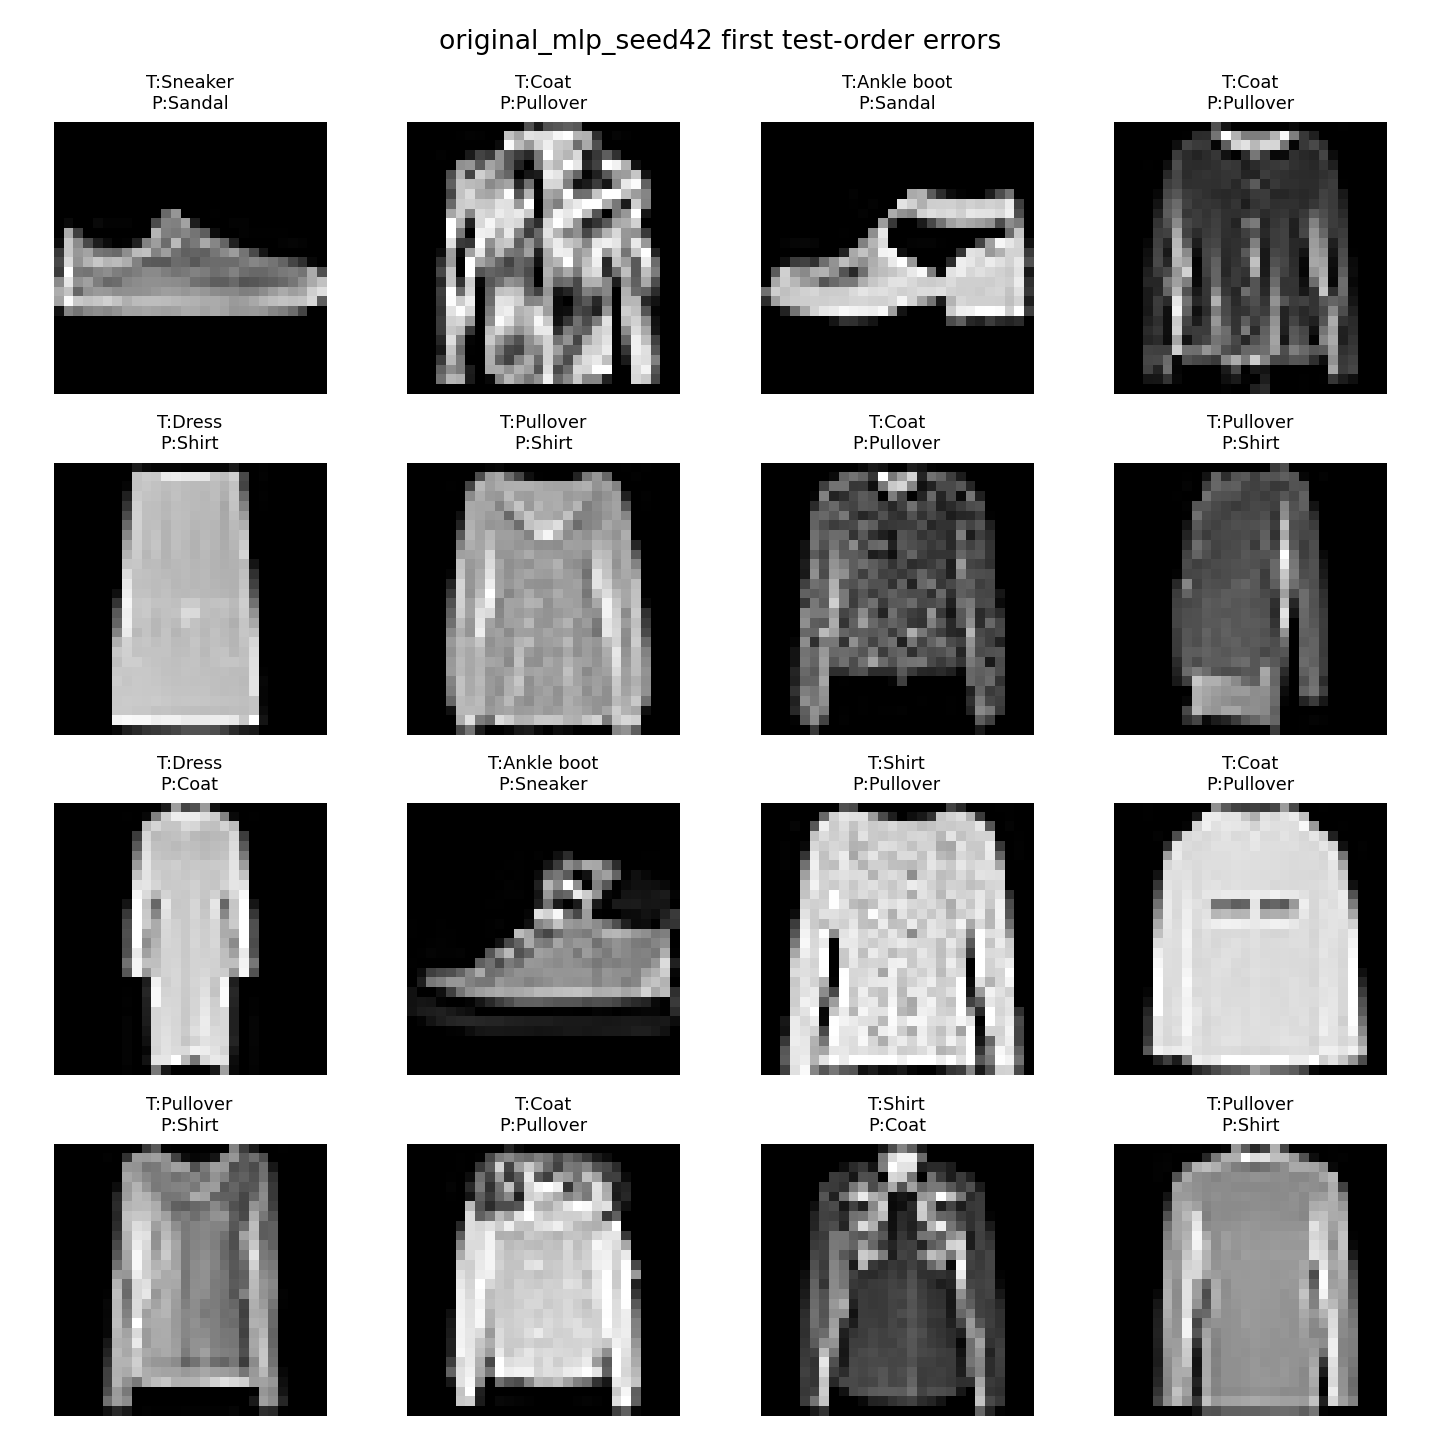
\includegraphics[width=\textwidth]{images/exp2/original_mlp_seed42_errors.png}
\end{minipage}\hfill
\begin{minipage}{0.48\textwidth}\centering
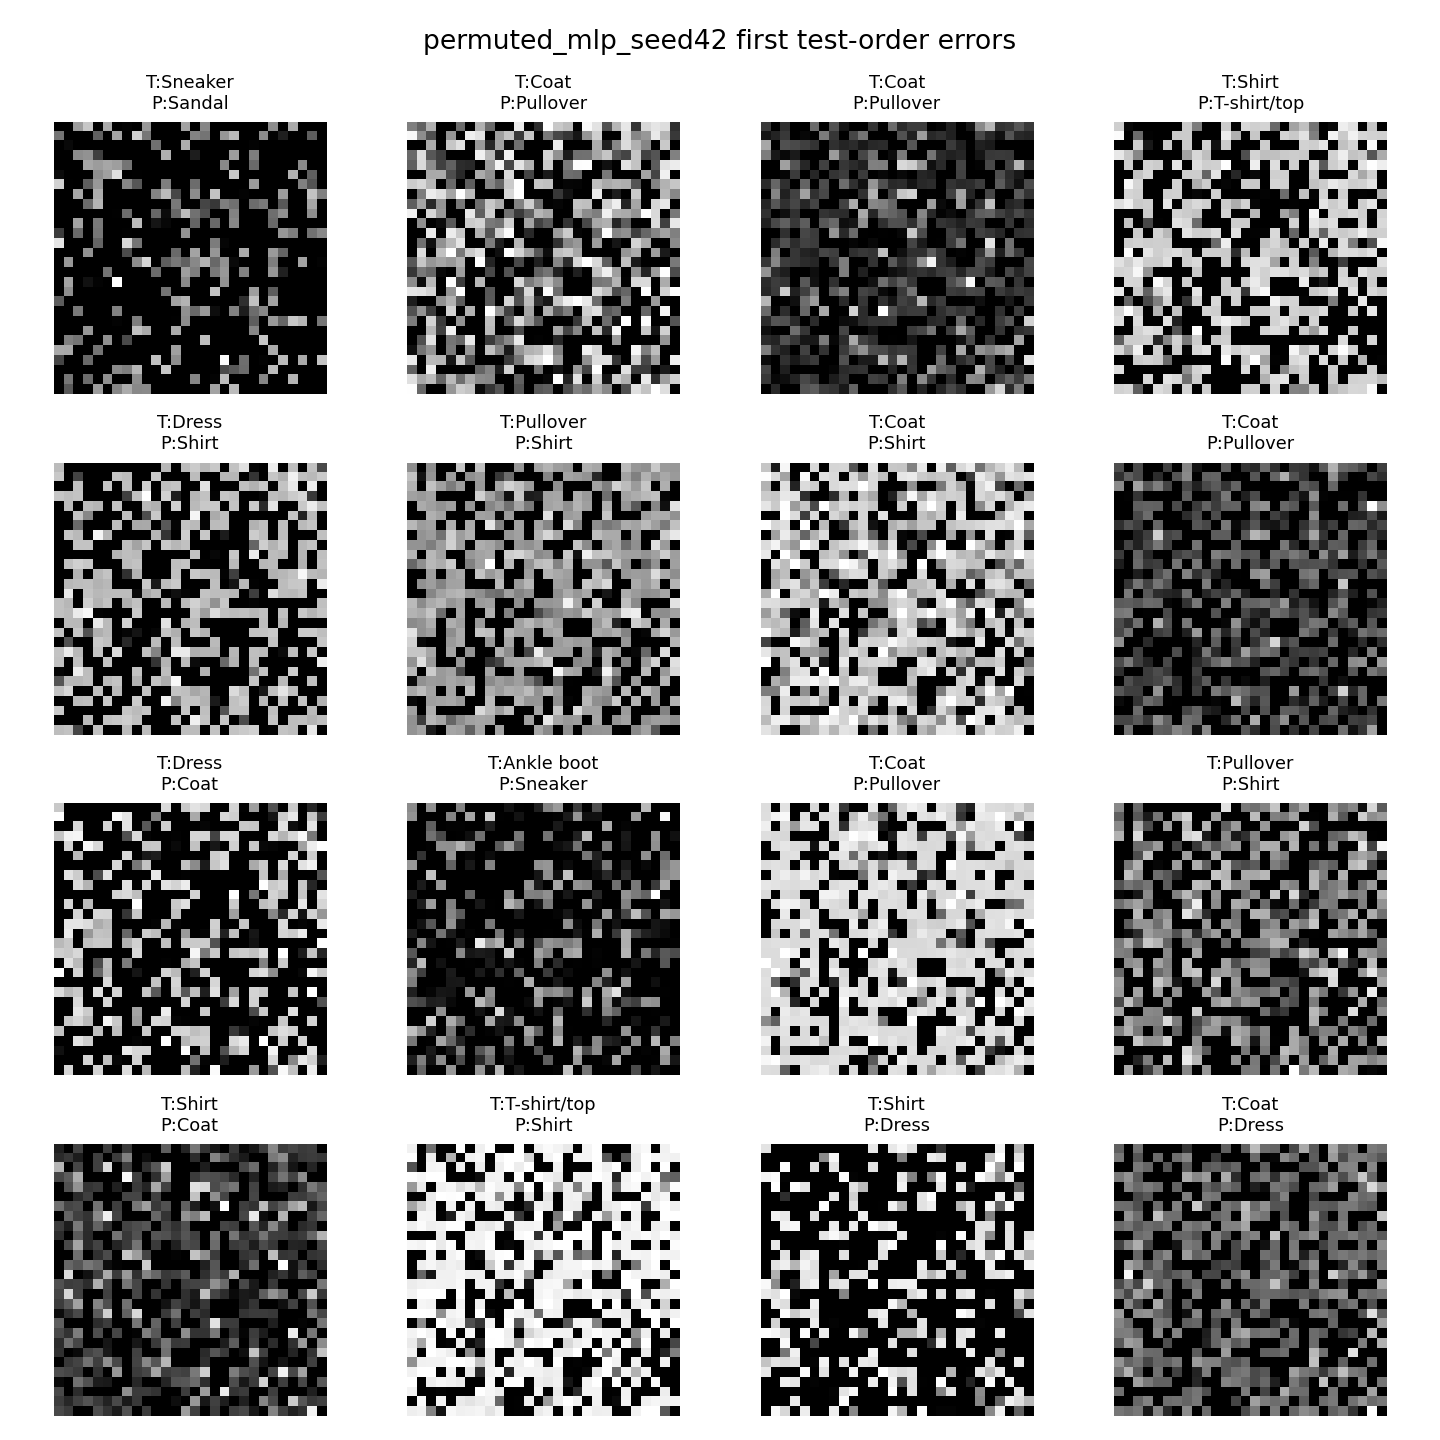
\includegraphics[width=\textwidth]{images/exp2/permuted_mlp_seed42_errors.png}
\end{minipage}
\caption{seed 42 的 MLP 测试错误：上为原图，下为置换图。每行均按测试索引顺序展示前 16 个错误}
\label{fig:mlp-errors}
\end{figure}

\subsection{固定像素置换实验}
使用 seed 20261024 生成一个 784 像素的固定置换，并将完全相同的置换用于训练、验证和测试图像。置换保留每张图的像素值与标签，只打乱像素的邻接关系。对照结果显示：置换使 CNN 测试准确率从 0.9189 降至 0.8788（下降 4.01 个百分点）；MLP 则从 0.8840 变为 0.8859（上升 0.19 个百分点，量级与种子波动相近）。置换后 CNN 比 MLP 低 0.71 个百分点；原图上 CNN 对 MLP 的 3.48 个百分点优势因此反转。这支持 CNN 的原图优势部分依赖局部空间结构先验，而非单纯由“参数更多”造成。

该结论有边界：这里只测试一个固定置换、三个训练种子；不同置换可能造成不同难度，且 CNN 仍达到 87.88\% 准确率，说明全局统计仍包含类别信息。置换条件训练时间比原图高约 20 秒（两种模型均如此），该差值可能受到输入置换处理和运行环境影响；模型间训练预算相同，但墙钟时间不应被解释为纯前向计算成本。\cref{fig:cm,fig:err} 对照 seed 42 的混淆矩阵与错误样本，可见原图错误主要仍是服饰间的语义近邻，而置换图样本已不具备直观轮廓。

\begin{figure}[H]
\centering
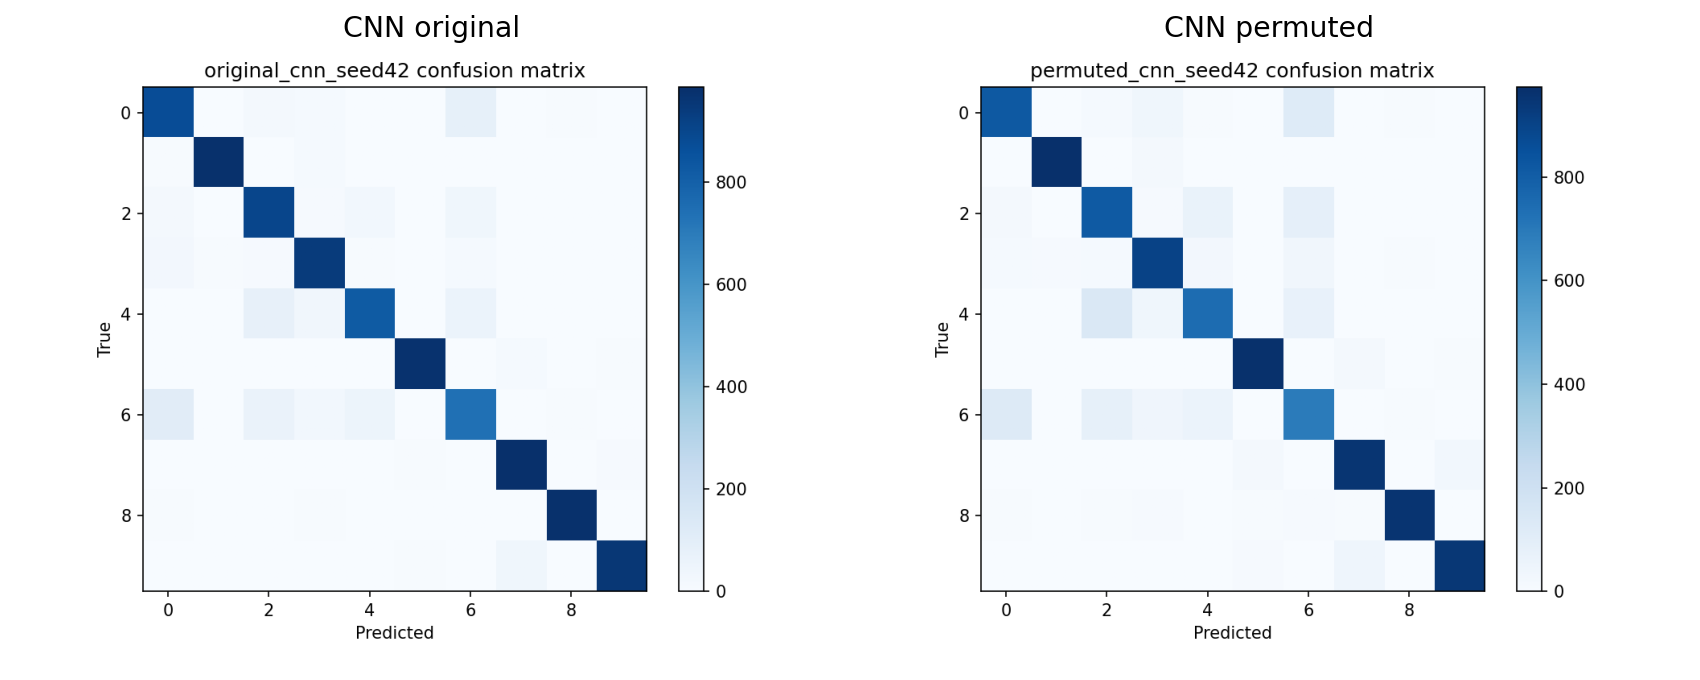
\includegraphics[width=0.76\textwidth]{images/exp2/cnn_confusions_pair.png}
\caption{CNN 测试混淆矩阵：左为原图，右为置换图。类别编号按 Fashion-MNIST 标准顺序 0--9}
\label{fig:cm}
\end{figure}

\begin{figure}[H]
\centering
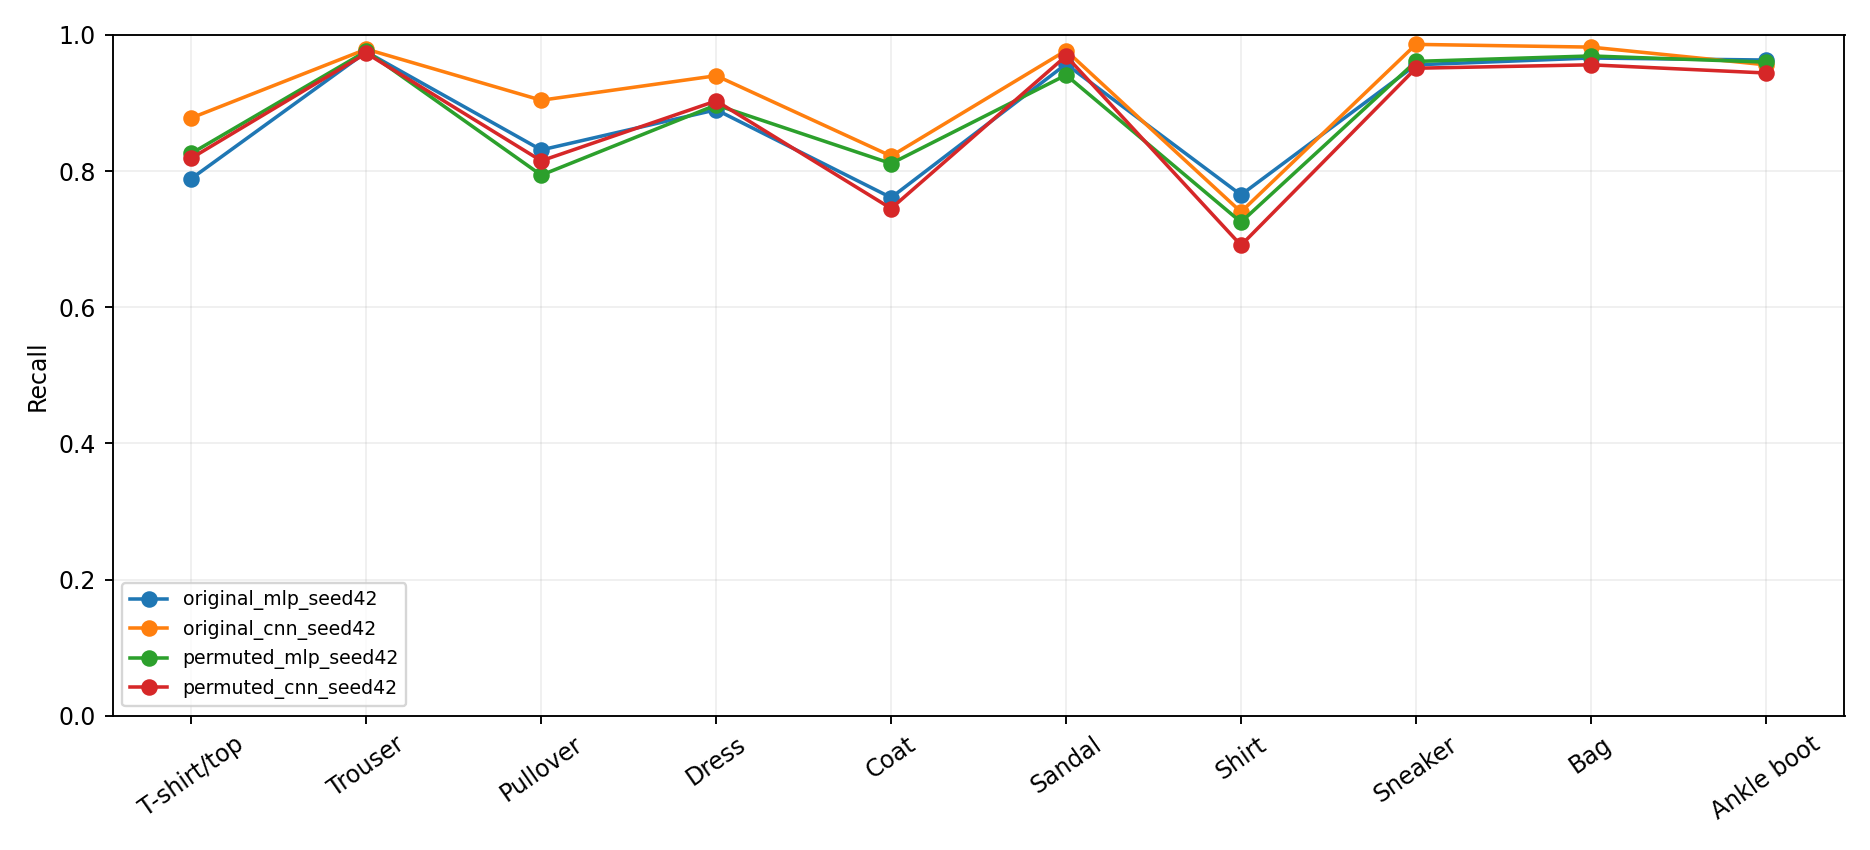
\includegraphics[width=0.76\textwidth]{images/exp2/per_class_recall.png}
\caption{四种输入/模型条件下的逐类召回率（seed 42）。各类别测试样本数相同，召回率可直接横向比较}
\label{fig:recall}
\end{figure}

逐类结果进一步细化了结构先验的作用。原图上 CNN 相对 MLP 在 T-shirt/top、Pullover 和 Coat 的召回率分别高约 8.9、7.3 和 6.1 个百分点，但 Shirt 低约 2.5 个百分点，Ankle boot 低约 0.7 个百分点。像素置换后，CNN 相对其原图的召回下降较多的类别包括 Pullover（约 8.9 个百分点）、Coat（约 7.7 个百分点）、T-shirt/top（约 5.9 个百分点）和 Shirt（约 4.9 个百分点）。整体准确率会掩盖类别差异；卷积局部先验主要改善若干视觉结构相似的服饰类别，并非对所有标签同等有效。

\section{扩散模型实现与训练}
本实验实现无条件 DDPM：给训练图像 $x_0$ 按预设噪声日程逐步加噪，令 $\alpha_t=1-\beta_t$、$\bar\alpha_t=\prod_{s=1}^t\alpha_s$，则
\[
 x_t=\sqrt{\bar\alpha_t}x_0+\sqrt{1-\bar\alpha_t}\,\epsilon,
 \qquad \epsilon\sim\mathcal{N}(0,I).
\]
去噪器接收 $x_t$ 和时间步 $t$（经时间步条件嵌入），学习预测噪声，目标为
\[
 \mathcal{L}_{\epsilon}=\mathbb{E}_{x_0,t,\epsilon}
 \left[\|\epsilon-\epsilon_\theta(x_t,t)\|_2^2\right].
\]
单步反向更新按 DDPM 噪声预测形式计算
\[
 x_{t-1}=\frac{1}{\sqrt{\alpha_t}}\left(x_t-
 \frac{\beta_t}{\sqrt{1-\bar\alpha_t}}\epsilon_\theta(x_t,t)\right)+\sigma_t z,
\]
其中 $z\sim\mathcal{N}(0,I)$（最后一步不再加噪）。完整采样从固定高斯噪声 $x_T$ 出发，按 $t=T,\ldots,1$ 迭代至 $x_0$\cite{ddpm}。模型不接收服饰类别条件。

\begin{table}[H]
\centering\small
\caption{扩散模型训练与采样记录}
\begin{tabular}{ll}
\toprule
训练样本数 & 50,000（固定训练子集） \\
基础通道数 / 参数量 & 32 / 148,673 \\
扩散步数 / epoch & 100 / 30 \\
设备 / 训练种子 & CUDA GPU / 42 \\
训练噪声 MSE & 0.4021（第 1 轮）$\to$ 0.1402（第 30 轮） \\
训练时间 & 129.58 秒 \\
采样种子 / 轨迹噪声种子 & 20261024 / 314159 \\
采样批量 / 记录时间 & 100 张 / 0.158--0.205 秒 \\
\bottomrule
\end{tabular}
\end{table}

训练日志中的噪声预测 MSE 总体下降并在约 0.14 附近趋缓；没有单独的扩散验证集损失，因此该曲线只说明训练目标被优化，不能单独证明生成分布质量。两份采样记录分别给出 0.158 秒和 0.205 秒/100 张，报告保留该实测范围（约 1.58--2.05 ms/张），反映短时 GPU 采样计时对同步与计时区间较敏感。训练种子、采样种子、轨迹噪声种子及初始噪声张量均有记录，固定噪声保存在扩散结果文件中。

\begin{figure}[H]
\centering
\begin{minipage}{0.47\textwidth}
\centering
\begin{tikzpicture}
\begin{axis}[width=\textwidth,height=4.1cm,xlabel=Epoch,ylabel=Noise-prediction MSE,grid=major,tick label style={font=\scriptsize},label style={font=\scriptsize}]
\addplot+[blue,mark=none] table[x=epoch,y=noise_mse,col sep=comma]{work/server_artifacts/results/exp2/diffusion/training_history.csv};
\end{axis}
\end{tikzpicture}
\captionof{figure}{扩散模型训练损失}
\end{minipage}\hfill
\begin{minipage}{0.50\textwidth}
\centering
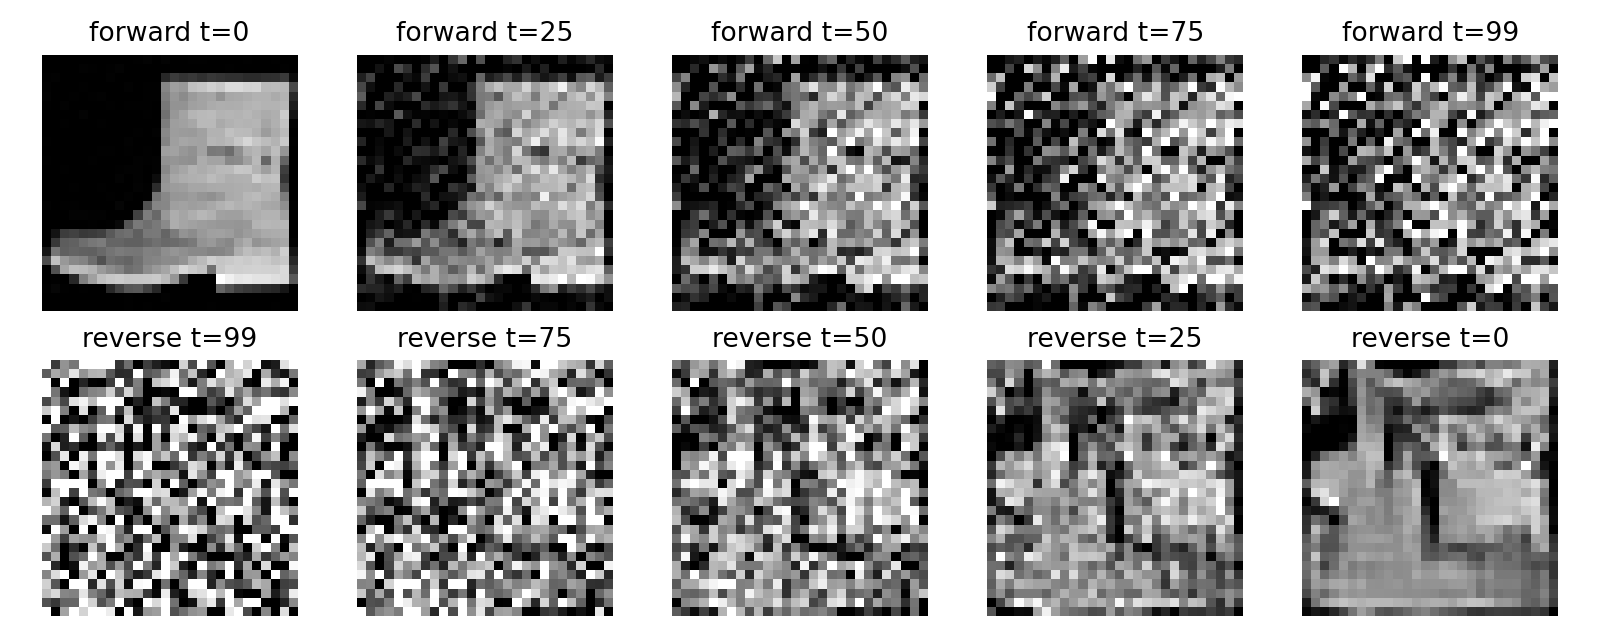
\includegraphics[width=\textwidth]{images/exp2/diffusion_process.png}
\captionof{figure}{固定样本的前向加噪与反向去噪过程}
\end{minipage}
\end{figure}

\clearpage
\section{生成质量评价与结论}
\cref{fig:grid} 展示固定采样种子生成的随机样本网格，非人工筛选的成功样本。训练集最近邻（\cref{fig:nearest}）从固定训练子集每 5 张取 1 张（10,000 张）中按原始像素 $L_2$ 距离搜索；该检查可以发现明显像素级复制，但不是感知距离，也不能排除子集之外的近邻。\cref{fig:coverage} 使用独立训练的 CNN 作为类别代理评价器，而非人工真值；100 张样本被预测为 Bag 86、Shirt 5、T-shirt/top 3、Trouser 3、Sandal 2、Pullover 1，其余四类为 0，仅覆盖 6/10 类。类别覆盖严重偏斜。代理分类器对这 100 张生成图的平均最大类别概率为 0.924；最低置信度四分位（25 张）的置信度均值为 0.730，范围为 0.478--0.900。高平均置信度与 86\% 样本集中在 Bag 并存，说明单看置信度会把模式塌缩误读为高质量。代理分类器只在真实 Fashion-MNIST 图像上训练，遇到模糊或异常生成图可能过度自信；类别计数是近似覆盖诊断，不是生成标签真值。最低置信度四分位的 25 张（\cref{fig:lowconf}）也全部展示，避免只呈现看起来较成功的样本。

\begin{figure}[H]
\centering
\begin{minipage}{0.35\textwidth}\centering
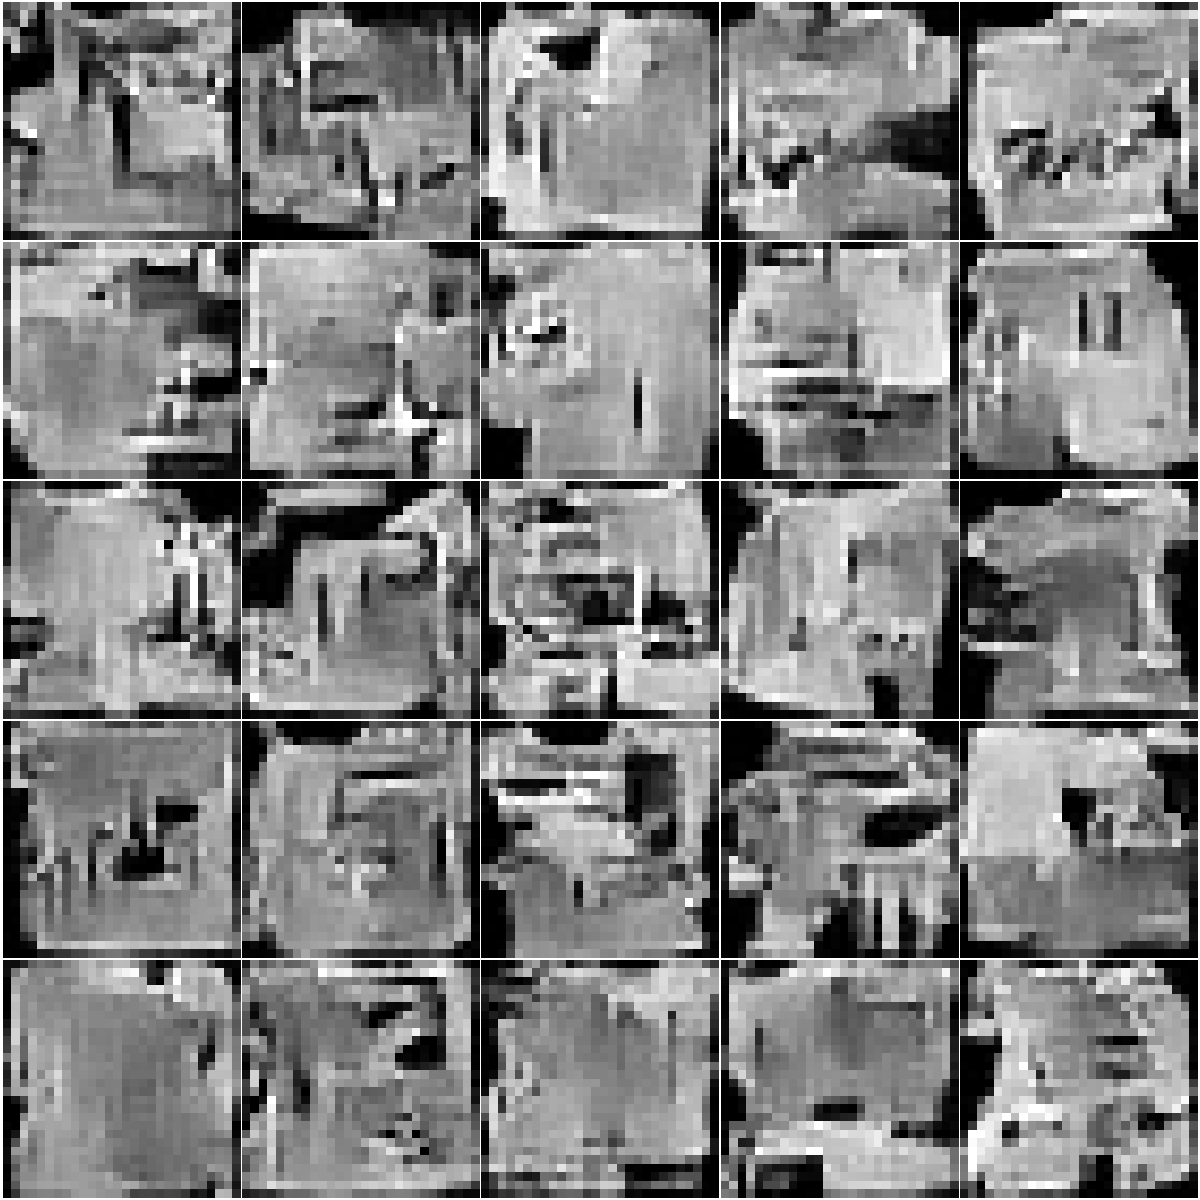
\includegraphics[width=0.9\textwidth,height=5.0cm,keepaspectratio]{images/exp2/diffusion_random_grid.png}
\captionof{figure}{固定初始噪声生成的随机样本网格}\label{fig:grid}
\end{minipage}\hfill
\begin{minipage}{0.50\textwidth}\centering
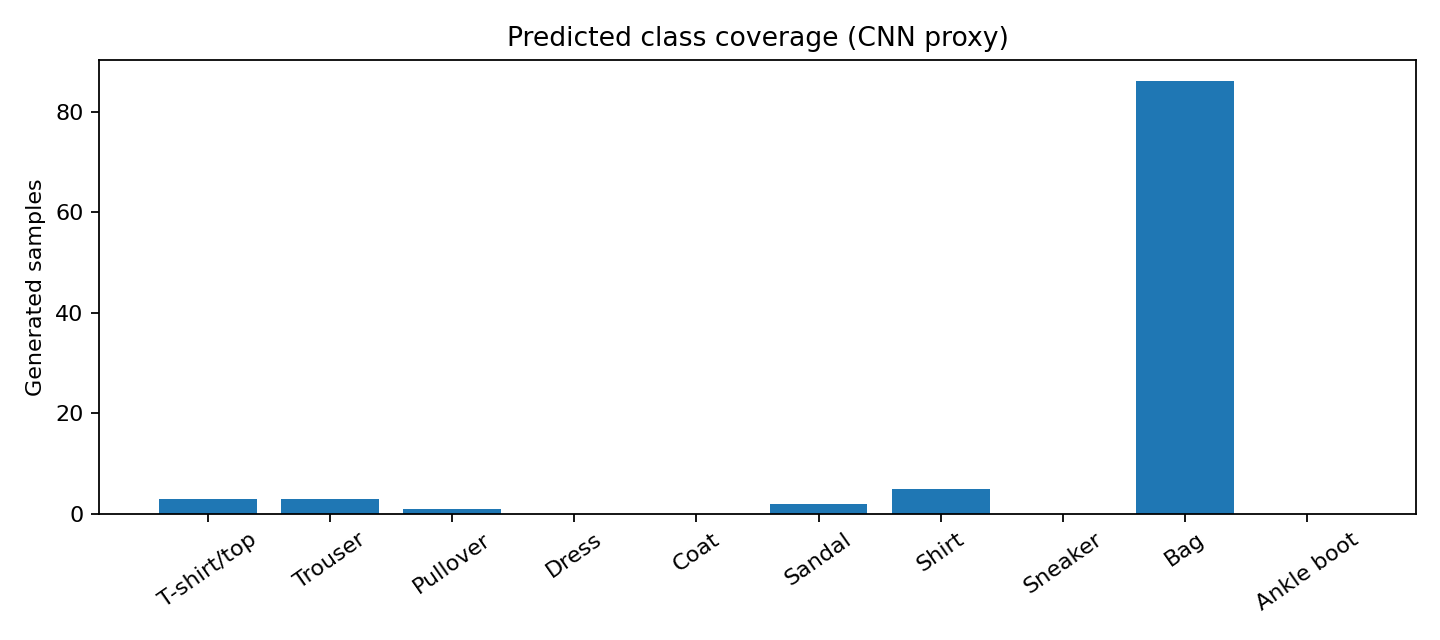
\includegraphics[width=\textwidth,height=3.2cm,keepaspectratio]{images/exp2/diffusion_class_coverage.png}
\captionof{figure}{100 张样本的代理类别覆盖}\label{fig:coverage}
\end{minipage}

\vspace{0.2em}
\begin{minipage}{0.40\textwidth}\centering
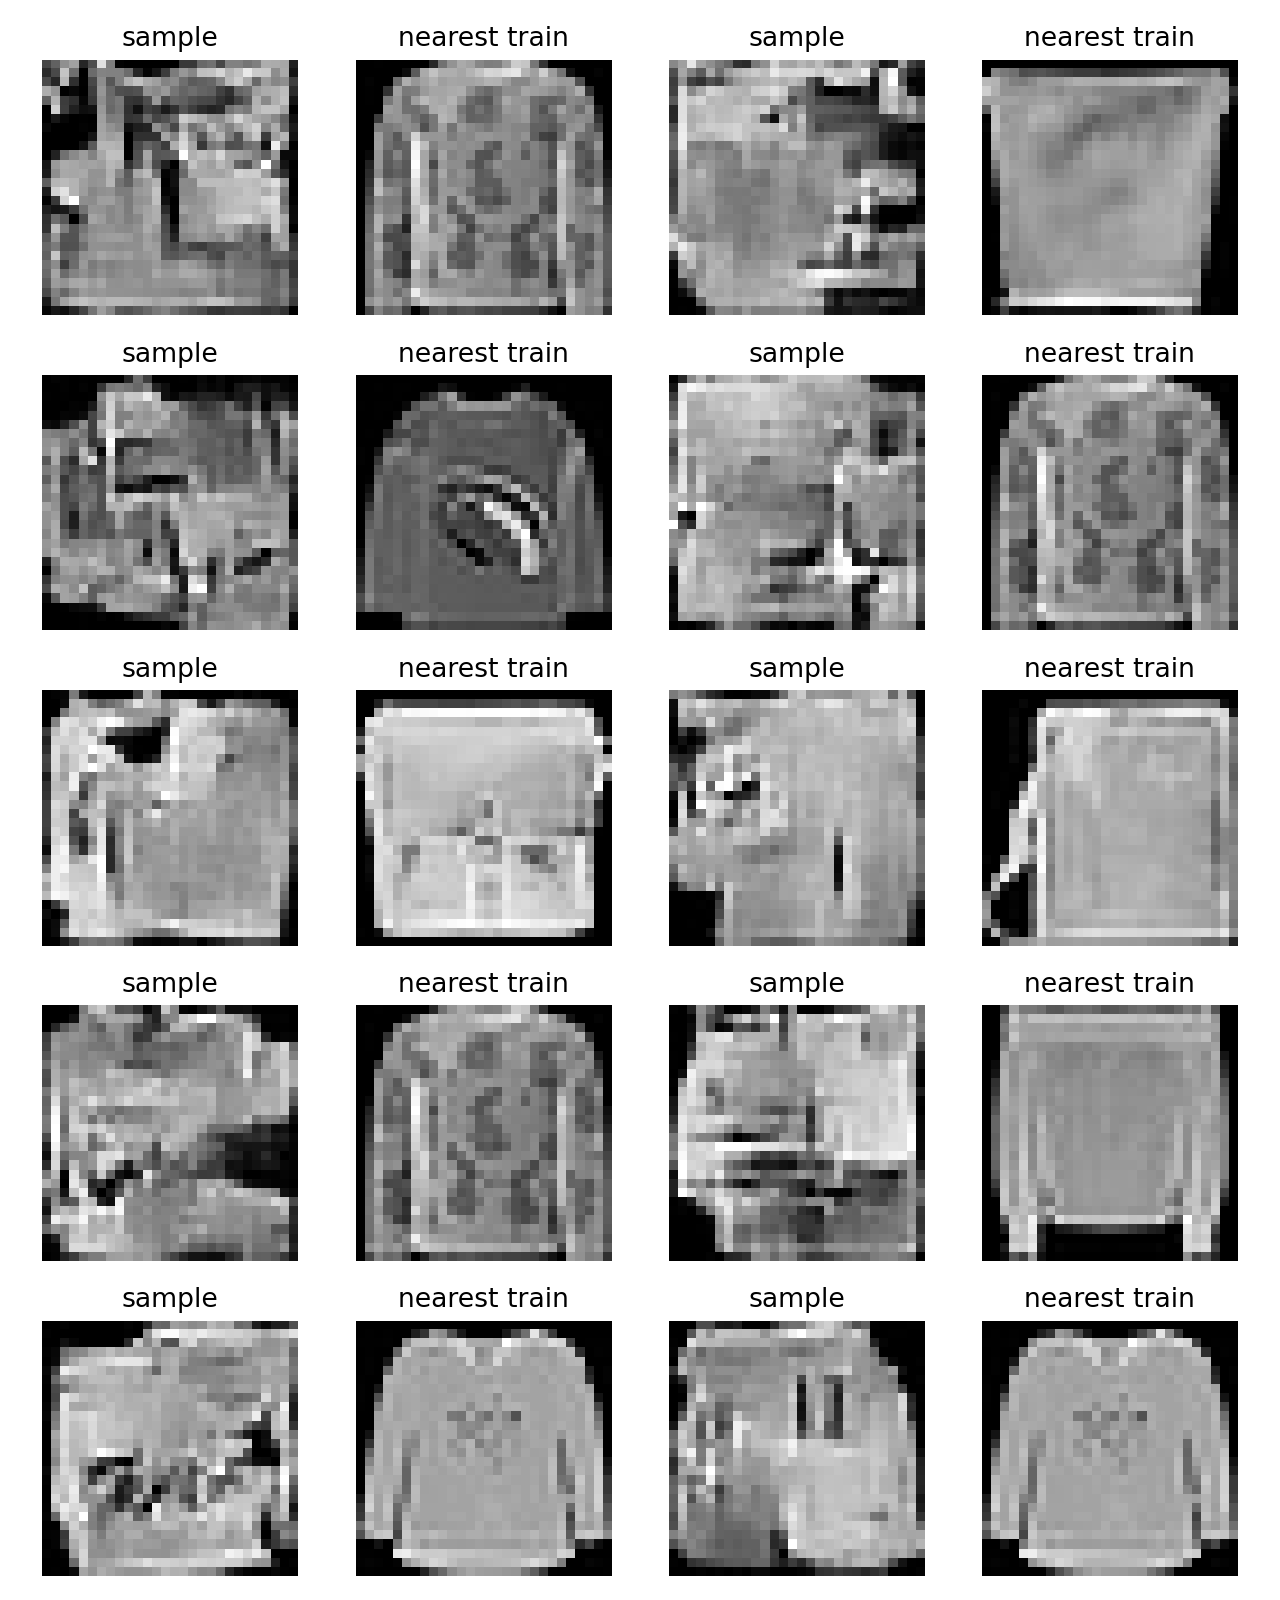
\includegraphics[width=\textwidth,height=7.0cm,keepaspectratio]{images/exp2/diffusion_nearest_neighbors.png}
\captionof{figure}{生成样本及训练子集像素距离最近邻}\label{fig:nearest}
\end{minipage}\hfill
\begin{minipage}{0.36\textwidth}\centering
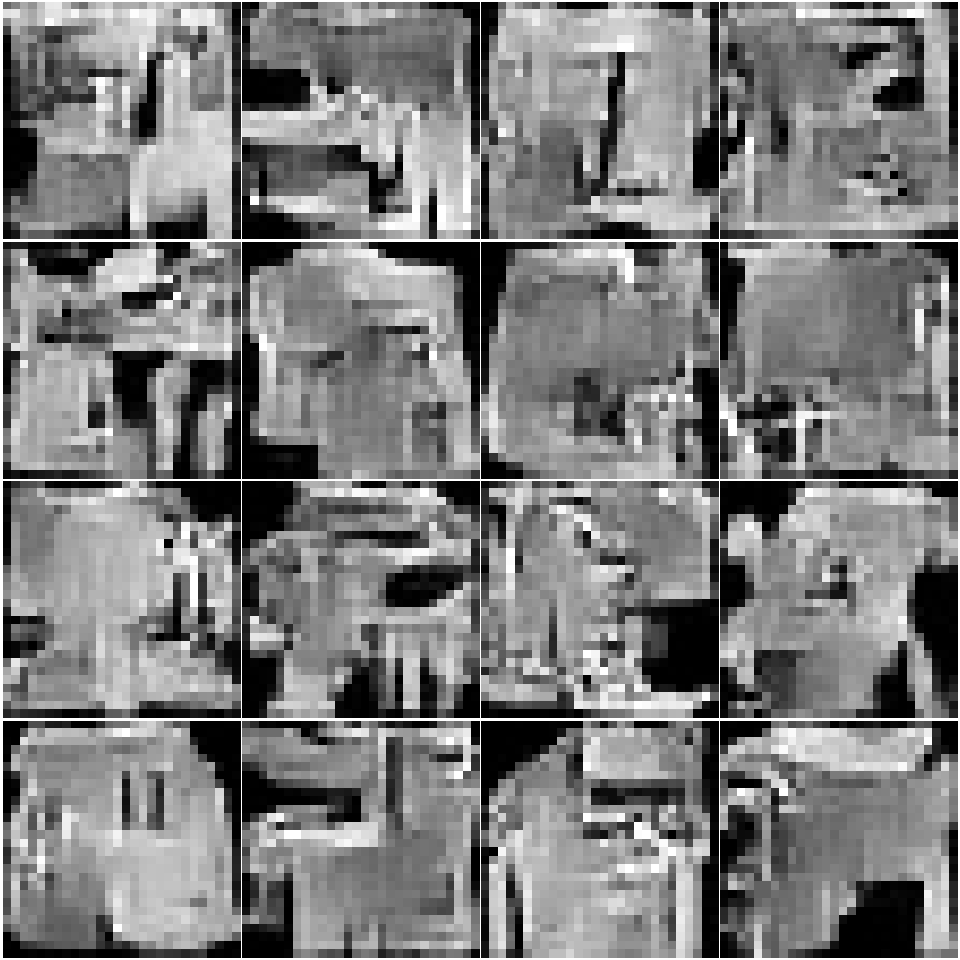
\includegraphics[width=\textwidth,height=5.3cm,keepaspectratio]{images/exp2/diffusion_low_confidence.png}
\captionof{figure}{固定批次中代理置信度最低的 25 张}\label{fig:lowconf}
\end{minipage}
\end{figure}

样本网格仍模糊且类别集中到 Bag，最近邻未显示清晰复制。扩散流程实现完整，但 30 轮训练未获得清晰、类别覆盖充分的样本。最近邻检索只覆盖固定 50,000 张训练样本中每隔五张取一张的 10,000 张子集，并在原始像素空间使用 $L_2$ 距离；它不能排除语义近邻或子集外的复制。生成任务无条件，类别统计依赖代理分类器；同时未设置独立的生成验证指标，也未比较网络规模、噪声日程或采样器。训练损失下降只能说明噪声回归目标得到优化，不能替代生成分布质量评价。分类结果支持 CNN 优势依赖原图局部空间结构；结论限于本实验模型、单一置换与三个种子。

\addcontentsline{toc}{section}{参考文献}
\begin{thebibliography}{9}
\bibitem{fashionmnist} H. Xiao et al. Fashion-MNIST. arXiv:1708.07747, 2017.
\bibitem{ddpm} J. Ho et al. Denoising Diffusion Probabilistic Models. NeurIPS, 2020.
\end{thebibliography}

\end{document}
